\documentclass[11pt]{article}
\usepackage[utf8]{inputenc}
\usepackage{float}
\usepackage{amsmath}
\usepackage{enumitem}

\usepackage[hmargin=3cm,vmargin=6.0cm]{geometry}
\topmargin=-2cm
\addtolength{\textheight}{6.5cm}
\addtolength{\textwidth}{2.0cm}
\setlength{\oddsidemargin}{0.0cm}
\setlength{\evensidemargin}{0.0cm}
\usepackage{indentfirst}
\usepackage{amsfonts}
\usepackage{wrapfig}
\usepackage[linguistics]{forest}
\usepackage{tikz}
\usetikzlibrary{arrows,automata,positioning}

\begin{document}

\section*{Student Information}

Name : Emre Geçit\\

ID : 2521581\\


\section*{Answer 1}

\paragraph{a)}Write a context-free grammar for the language $L_1 = \{w | w \in \{a, b\}^* \wedge  \text{ w has twise as many b's as a's}\}$.\\\\
Let $G$ be the grammar $(V, \Sigma, R, S)$ for the language $L_1$ where
\begin{flalign*}
         V = \{&S, a, b\},\\
    \Sigma = \{&a, b\},\\
         R = \{&S \rightarrow aSbSb,\\
               &S \rightarrow bSaSb,\\
               &S \rightarrow bSbSa,\\
               &S \rightarrow e\}.
\end{flalign*}
\paragraph{b)}Write a context-free grammar for the language $L_2 = \{a^nb^m | m, n \in \mathbb{N}  \wedge m \leq n \leq 2m\}$.\\\\
Let $G$ be the grammar $(V, \Sigma, R, S)$ for the language $L_2$ where
\begin{flalign*}
         V = \{&S, a, b\},\\
    \Sigma = \{&a, b\},\\
         R = \{&S \rightarrow aSb,\\
               &S \rightarrow aSbb,\\
               &S \rightarrow e\}.
\end{flalign*}
\newpage
\paragraph{c)}Formally define and draw a PDA that accepts $L_1$.\\\\
Let $(K, \Sigma, V, \Delta, p, \{q\})$ be the sextuple for the language $L_1$ where $K$, $\Sigma$, $V$, $R$ are defined on part a.

$\Delta$ contains the following transitions:
\begin{enumerate}[label=\arabic*)]
    \item $((p, e, e), (q, S))$
    \item $((p, e, A), (q, x))$ for each rule $A \rightarrow x$ in $R$
    \item $((q, a, a), (q, e))$ for each $a \in \Sigma$
\end{enumerate}
\begin{wrapfigure}{r}{0.57\textwidth}
     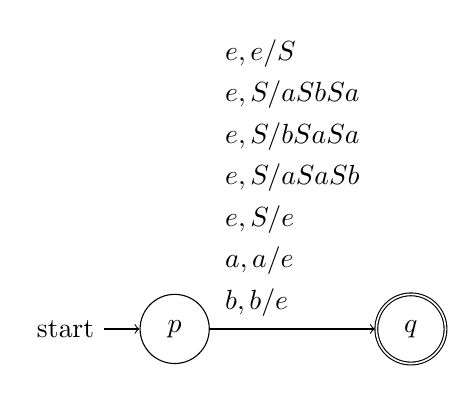
\begin{tikzpicture}[->,auto,node distance=3cm]
     
     \node[initial,state] (p)                    {$p$};
     \node[state, accepting]         (q) [right of=p]       {$q$};
     
     \path (p) edge              node {$\begin{aligned}
                    &e, e / S\\
                    &e, S / aSbSa\\
                    &e, S / bSaSa\\
                    &e, S / aSaSb\\
                    &e, S / e\\
                    &a, a / e\\
                    &b, b / e
      \end{aligned}$} (q)

     ;
     \end{tikzpicture}
\end{wrapfigure}

Then, \begin{flalign*}
    \Delta = \{&((p, e, e), (q, S)),\\
               &((p, e, S), (q, aSbSa)),\\
               &((p, e, S), (q, bSaSa)),\\
               &((p, e, S), (q, aSaSb)),\\
               &((p, e, S), (q, e)),\\
               &((p, a, a), (q, e)),\\
               &((p, b, b), (q, e))\}.
\end{flalign*}\\\\

\paragraph{d)}Write a context-free grammar for the language $L_3 = L_1 \cup  L_2.$\\\\
Let $G_1 = (V_1, \Sigma_1, R_1, S_1)$ for the language $L_1$ and $G_2 = (V2, \Sigma_2, R_2, S_2)$ for the language $L_2$.\\\\
Then $G_3 = (V_1 \cup V2 \cup \{S\}, \Sigma_1 \cup \Sigma_2, R_1 \cup R_2 \cup \{S \rightarrow S_1, S \rightarrow S_2\})$ for the language $L_3$.\\\\
\begin{flalign*}
       V_3 = \{&S, S_1, S_2, a, b\}\\
    \Sigma = \{&a, b\}\\
         R = \{&S \rightarrow S_1,\\
               &S \rightarrow S_2,\\
               &S_1 \rightarrow aS_1bS_1b,\\
               &S_1 \rightarrow bS_1aS_1b,\\
               &S_1 \rightarrow bS_1bS_1a,\\
               &S_1 \rightarrow e,\\
               &S_2 \rightarrow aS_2b,\\
               &S_2 \rightarrow aS_2bb,\\
               &S_2 \rightarrow e\}.
\end{flalign*}
\section*{Answer 2}
Given $G_1 = \{V, \Sigma, R, S\}$ where $V = \{0,1, S, A\}$ , $\Sigma = \{0,1\}$ , and $R = \{S \rightarrow AS |e , A \rightarrow A1 | 0A1 | 01\}$
\paragraph{a)}Show that $G_1$ is ambiguous.\\\\
For the string $00111$, there are more than one possible rightmost derivations.
\begin{enumerate}[label=\arabic*)]
     \item $S \rightarrow AS \rightarrow A \rightarrow 0A1 \rightarrow 0A11 \rightarrow 00111$
     \item $S \rightarrow AS \rightarrow A \rightarrow A1 \rightarrow 0A11 \rightarrow 00111$
\end{enumerate}
\paragraph{b)}Give an unambiguous grammar for $L(G_1)$. (i.e. disambiguate the given grammar.)\\\\
The reason why this grammar is ambiguous is that whenever the derivation includes the rules $A \rightarrow 0A1$ and $A \rightarrow A1$ these rules' application order can be swapped without affecting the final string. This issue can be solved in a way that restricts the application order of the rules. For this purpose, we will define a new nonterminal $B$, and define a transition from $A$ to $B$. After some modifications, $G_1$ is as follows:
\begin{flalign*}
     V = \{&S, A, B, 0, 1\}\\
\Sigma = \{&0, 1\}\\
     R = \{&S \rightarrow AS,\\
           &S \rightarrow e,\\
           &A \rightarrow 0A1,\\
           &A \rightarrow B,\\
           &B \rightarrow B1,\\
           &B \rightarrow 01\}
\end{flalign*}

\paragraph{c)}Give the leftmost derivation of the string 00111 from the grammar you have constructed at part-b
and draw the corresponding parse tree.\\\\
$S \rightarrow AS \rightarrow 0A1S \rightarrow 0B1S \rightarrow 0B11S \rightarrow 00111S \rightarrow 00111$\\\\
\begin{forest}
     [\textit{$S$}
       [\textit{$A$}
           [\textit{$0$}]
           [\textit{$A$}
               [\textit{$B$}
                   [\textit{$B$}
                       [\textit{$0$}]
                       [\textit{$1$}]
                   ]
                   [\textit{$1$}]
               ]
           ]
           [\textit{$1$}]
       ]
       [\textit{$e$}]
     ]
   \end{forest}
\end{document}